\documentclass[a4paper]{article}
\usepackage[welsh]{babel}
\selectlanguage{welsh}

\usepackage{hyperref}

% Set up page size
\usepackage[margin=1.5cm, includefoot, footskip=30pt]{geometry}

% Nice way to display code
\usepackage{minted}

% Import images
\usepackage{graphicx}
\usepackage{amsmath}
\usepackage{multicol}

\usepackage{tikz}
\usetikzlibrary{calc}

\title{Modelu effaith brechiadau gyda hafaliadau differol}
\author{Vince Knight}
\date{}


\begin{document}
\maketitle


\section{Cyflwyniad}\label{sec:introduction}

Mae Sefydliad Iechyd y Byd yn amcangyfrif bod y brechiad ar gyfer y frech goch
wedi arbed dros 17 miliwn o fywydau ers 2000~\cite{who}. Mae'n bosib modelu
effaith y brechiadau gan ddefnyddio hafaliadau differol. Fe elwir y model a
ystyriwn yn fodel SIR sy'n fodel rhannol o bobl heintiedig  all fod mewn un o 3
cyflwr:

\begin{itemize}
    \item Tueddol (S): aelodau o'r boblogaeth a all cael eu heintio;
    \item Heintiedig (I): aelodau heintiedig o'r boblogaeth y bydd yn adfer o'r
    afiechyd;
    \item Wedi'u Hadfer (R): aelodau o'r boblogaeth sydd wedi adfer o'r afiechyd,
    nodwch fan hyn mae marwolaeth yn fathemategol yn gyfath i adferiad.
\end{itemize}

Mae Darlun~\ref{fig:sir_model} yn dangos hwn fel diagram.

\begin{figure}[!hbtp]
    \begin{center}
        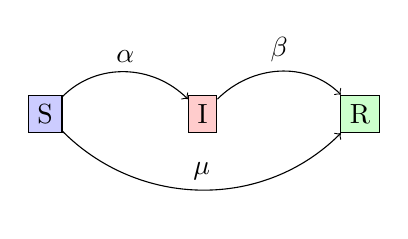
\begin{tikzpicture}
            \node [draw, fill=blue!20] (S) at (0, 0) {S};
            \node [draw, fill=red!20] (I) at ($(S) + (2, 0)$) {I};
            \node [draw, fill=green!20] (R) at ($(I) + (2, 0)$) {R};

            \draw [->] (S) edge [out=45, in=135] node [above] {\(\alpha\)} (I);
            \draw [->] (I) edge [out=45, in=135] node [above] {\(\beta\)} (R);
            \draw [->] (S) edge [out=-45, in=-135] node [above] {\(\mu\)} (R);
        \end{tikzpicture}
    \end{center}
    \caption{Y model SIR}
    \label{fig:sir_model}
\end{figure}

Parametrau'r model a ddangosir yn Darlun~\ref{fig:sir_model} yw:

\begin{itemize}
    \item \(\alpha\) y gyfradd heinti;
    \item \(\beta\) y gyfradd adfer;
    \item \(\mu\) y canran brechu;
\end{itemize}

Fe ellir mynegi hwn yn fathemategol:

\begin{align}
    \frac{dS}{dt} &= - \alpha I S - \mu S\\
    \frac{dI}{dt} &=  \alpha I S - \beta I\\
    \frac{dR}{dt} &=  \mu S + \beta I
\end{align}

Yn yr adran nesaf defnyddiwn Sympy i geisio datrys yr hafaliadau hyn yn
analytig.


\section{(Dim yn) canfod datrysiad union}

Mae'n bosib defnyddio Sympy i ddatrys systemau o hafaliadau differol, ond wrth
geisio ei wneud fan hyn mae i'w weld i fethu:

\begin{minted}{python}
>>> import sympy as sym
>>> S, I, R = sym.Function("S"), sym.Function("I"), sym.Function("V")
>>> N, mu, alpha, beta, t = sym.symbols("N, mu, alpha, beta, t")
>>> eq1 = sym.Derivative(S(t), t) - (- alpha * S(t) * I(t) - mu * R(t))
>>> eq2 = sym.Derivative(I(t), t) - (alpha * I(t) * S(t) / N  - beta * I(t))
>>> eq3 = sym.Derivative(R(t), t) - (beta * I(t) + mu * R(t))
>>> sym.dsolve((eq1, eq2, eq3))
NotImplementedError                       Traceback (most recent call last)
...
\end{minted}

Credaf fod hyn oherwydd cymhlethdod yr hafaliadau differol ac nid yw Sympy yn
gallu ei thrin yn analytig. Cafwyd datrysiad union heb ddefnyddio brechiadau
yn~\cite{harko2014exact}.
Serch hynny, yn yr adran nesaf byddwn yn eu datrys yn rhifiadol.


\section{Datrys yr hafaliadau yn rhifiadol ac effaith  y cyfradd brechu}

Gallwn ddefnyddio techneg integru rifiadol er mwyn datrys yr hafaliadau yn
rhifiadol. Disgrifir yr algorithm penodol a defnyddiwyd yn y cyhoeddiad
technegol~\cite{radhakrishnan1993description}.


Yn gyntaf cr\"{e}wn ffwythiant sy'n rhoi mynegiadau ar gyfer y deilliadau ar
gyfer unrhyw bwynt mewn amser:

\begin{minted}{python}
>>> def dx(x, t, alpha, beta, mu):
...     return (- alpha * x[1] * x[0] - mu * x[0],
...             alpha * x[1] * x[0]  - beta * x[1],
...             beta * x[1] + mu * x[0])
\end{minted}

Yna gallwn blotio nifer o senarios gwahanol fel y dangosir yn
Ddarlun~\ref{fig:scenarios}. Dyma'r cod sy'n cyfateb \^{a}'r plot cyntaf:

\begin{minted}{python}
>>> alpha = 1 / 1000  # Mae pob 1000 rhyngweithrediadu yn arwain at haint
>>> beta = 1 / 5  # Mae'n cymryd 5 uned amser i adfer o'r afiechyd
>>> N = 10 ** 4  # Poblogaeth o 10 mil o bobl
>>> mu = 0  # 0 canran brechu
>>> ts = np.linspace(0, 10, 5000)
>>> xs = integrate.odeint(func=dx, y0=np.array([N - 1, 1, 0]), t=ts, args=(alpha, beta, mu))
>>> S, I, R = xs.T
>>> plt.figure()
>>> plt.plot(ts, S, label="Tueddol")
>>> plt.plot(ts, I, label="Heintiedig")
>>> plt.plot(ts, R, label="Wedi Adfer")
>>> plt.legend()
>>> plt.title(f"$\max(I)={round(max(I))}$ ($\\alpha={alpha}$, $\\beta={beta}$, $\mu={mu}$)")
>>> plt.savefig("base_scenario.pdf");
\end{minted}

\begin{figure}[!hbtp]
    \begin{center}
        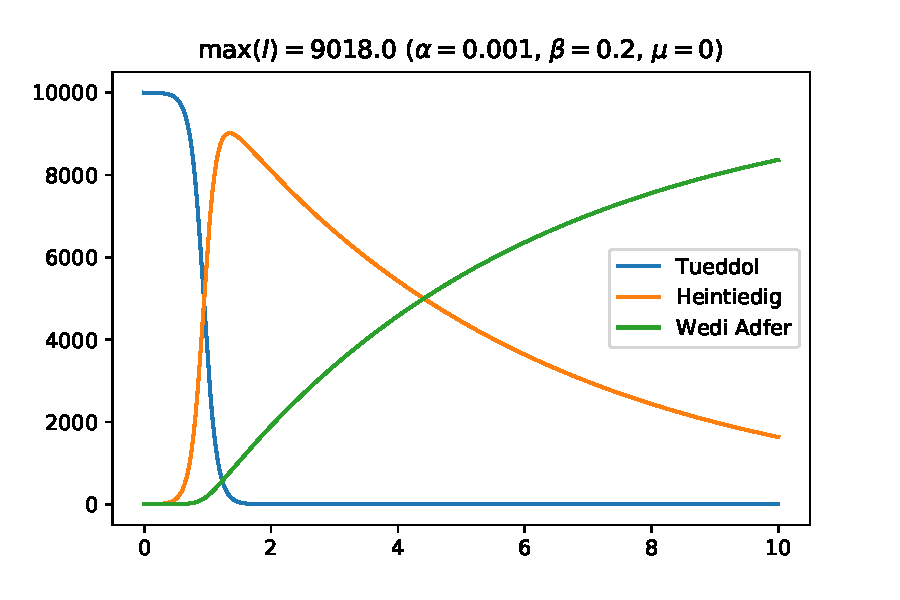
\includegraphics[width=.3\textwidth]{base_scenario.pdf}
        ~
        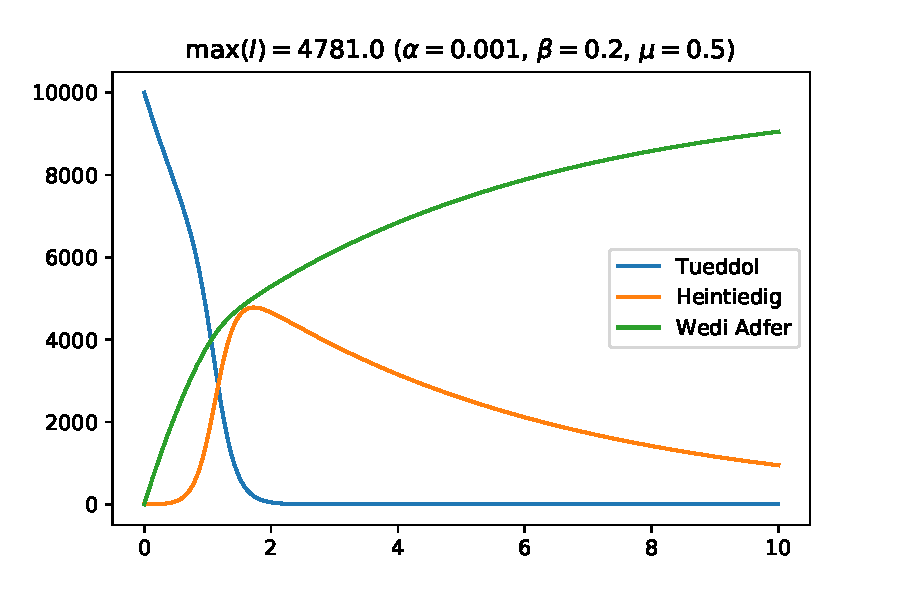
\includegraphics[width=.3\textwidth]{moderate_vaccination_rate.pdf}
        ~
        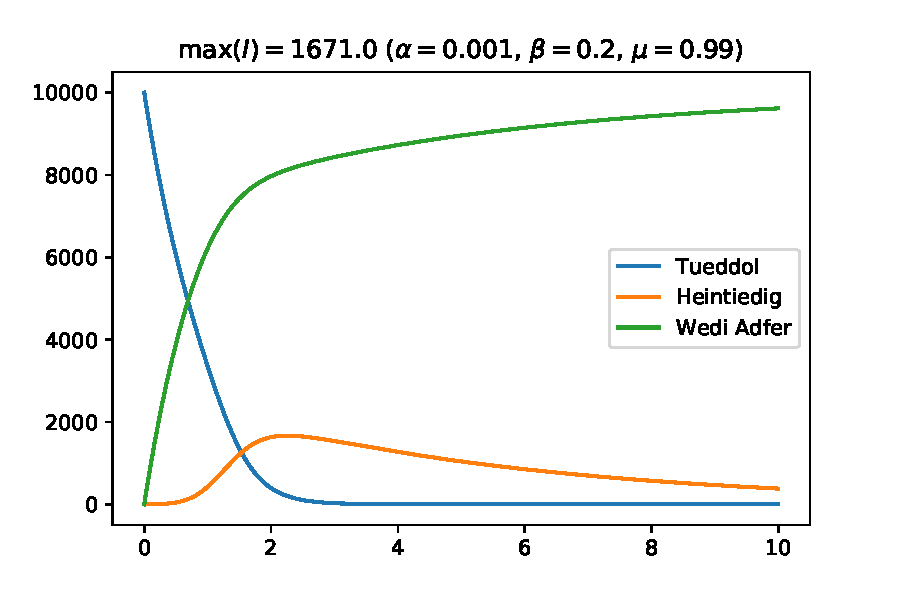
\includegraphics[width=.3\textwidth]{high_vaccination_rate.pdf}
        \caption{Esblygiad y boblogaeth ar gyfer canrannau gwahanol ar gyfer brechiadau}
        \label{fig:scenarios}
    \end{center}
\end{figure}

Mae hefyd yn bosib cyfrifo uchafswm y canran heintio fel ffwythiant o'r gyfradd
brechu:

\begin{minted}{python}
>>> vaccination_rates = np.linspace(0, 1, 500)
>>> max_percent_of_infected = []
>>> for mu in vaccination_rates:
...     xs = integrate.odeint(func=dx, y0=np.array([N - 1, 1, 0]), t=ts, args=(alpha, beta, mu))
...     S, I, R = xs.T
...     max_percent_of_infected.append(max(I) / N)
>>> plt.figure()
>>> plt.plot(vaccination_rates, max_percent_of_infected)
>>> plt.xlabel("$\mu$")
>>> plt.ylabel("% o'r poblogath sy'n heintiedig")
>>> plt.savefig("effect_of_vaccination_rate.pdf");
\end{minted}

Dangosir hwn yn Ddarlun~\ref{fig:effect_of_vaccination_rate}.

\begin{figure}[!hbtp]
    \begin{center}
        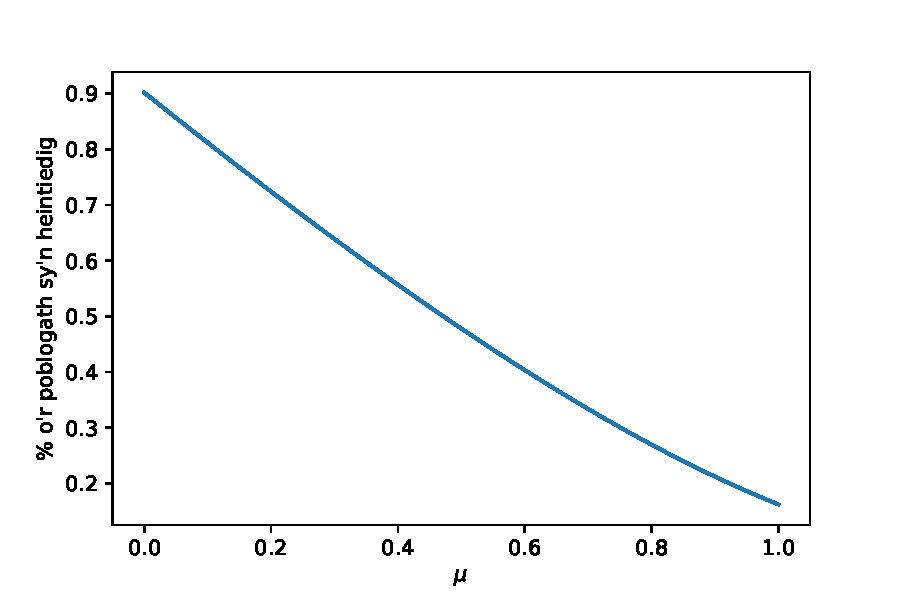
\includegraphics[width=.6\textwidth]{effect_of_vaccination_rate.pdf}
        \caption{Effaith y cyfradd brechu ar uchafswm y canran heintio}
        \label{fig:effect_of_vaccination_rate}
    \end{center}
\end{figure}

\section{Casgliad}

Gwelwn yn ein model bod angen cyfradd brechu mawr er mwyn sicrhau lefel uchel o
imiwnedd (hy lefel macsimwm isel o gyfanswm heintio). Mae'r fath yma o ddull yn
defnyddio hafaliadau differol i fodelu rhyngweithiadau unigolion a lledaeniad
afiechyd, yn olaf datryswn ni'r hafaliadau hyn gan ddefnyddio technegau o
ddadansoddi rhifiadol.

\bibliographystyle{plain}
\bibliography{bibliography.bib}

\end{document}
